\documentclass{article}
\usepackage[utf8]{inputenc}
\usepackage{listings}
\usepackage{xcolor}
\usepackage{graphicx}
\usepackage{amsmath}
\usepackage{float}
\usepackage{hyperref}
\graphicspath{ {./images/} }
\usepackage{algorithm}
\usepackage{algorithmic}
%New colors defined below
\definecolor{codegreen}{rgb}{0,0.6,0}
\definecolor{codegray}{rgb}{0.5,0.5,0.5}
\definecolor{codepurple}{rgb}{0.58,0,0.82}
\definecolor{backcolour}{rgb}{0.95,0.95,0.92}

%Code listing style named "mystyle"
\lstdefinestyle{mystyle}{
  backgroundcolor=\color{backcolour},   commentstyle=\color{codegreen},
  keywordstyle=\color{magenta},
  numberstyle=\tiny\color{codegray},
  stringstyle=\color{codepurple},
  basicstyle=\ttfamily\footnotesize,
  breakatwhitespace=false,         
  breaklines=true,                 
  captionpos=b,                    
  keepspaces=true,                 
  numbers=left,                    
  numbersep=5pt,                  
  showspaces=false,                
  showstringspaces=false,
  showtabs=false,                  
  tabsize=2
}

%"mystyle" code listing set
\lstset{style=mystyle}

\title{Advanced Binary Search}
\author{Nikhil Pesaladinne, Sauman Das }
\date{April 2021}

\begin{document}

\maketitle

\section{Introduction}
Most people already know the basic application of binary search which is to find the position of a value in a sorted list. We will review the basic algorithm, however, there are many other useful applications of this simple algorithm. Let's start by reviewing the basics. 

\section{Basic Binary Search}\label{intro}
Binary search works by repeatedly dividing the search interval in half, eventually arriving to the wanted value. You begin by the interval covering the entire array, if the wanted value is lower than the middle of the interval, search the lower half of the interval, and if it is higher, then search the upper half. We then repeat this process until we arrive to the wanted value. If our interval's size ever reaches $0$ however, we know that the wanted value does not exist in our array.

\begin{lstlisting}[language=Java, title=Binary Search Psuedocode]
    low = 1;
		high = n;
		target = x;
		
		while(target not found)
		{
			if(high < low)
				x does not exist
			mid = low + (high - low + 1)/2;
			if(array[mid] < x)
				low = mid + 1
			if(array[mid] > x)
				high = mid - 1
			if(array[mid] == x)
				x is at array[mid]
		}
\end{lstlisting}

The above implementation is one that most people are familiar with. There is another way to search through an array with the same average time complexity often referred to by the name ``jump searching". This search involves setting certain intervals to search through an array. When you overshoot your target value, the interval size is halved so that a narrower search can be conducted. 

\begin{algorithm}
\label{alg:jump}
\caption{Searching by Jumps}
\begin{algorithmic}[1]  
\STATE $intervalSize \leftarrow hi-lo$
\WHILE{$intervalSize > 0$}
\WHILE{$inBound(lo+intervalSize)~\text{and}~check(lo+intervalSize)$}
\STATE $lo \leftarrow lo+intervalSize$
\ENDWHILE
\STATE $intervalSize \leftarrow intervalSize/2$
\ENDWHILE
\RETURN lo
\end{algorithmic}
\end{algorithm}

Using the jumps implementation can sometimes be shorter in terms of writing code. However, both are equally efficient and take $\mathcal{O}(\log(n))$ time.

Using this algorithm, we can easily and efficiently find whether an element exists in an array. However, sometimes we may want more than just that.
\section{Variations of Binary Search}
\subsection{Binary Search on a rotated Array}
\textbf{Problem: } Given a sorted array of distinct elements, and the array is rotated at an unknown position. Find minimum element in the array.

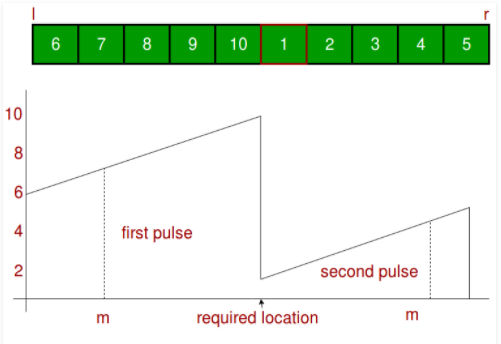
\includegraphics{rotatedbinarysearch.png}

We define $l$ and $r$ to be the left and right endpoints of our search interval respectively. Let $m$ be the middle position between $l$ and $r$. How can we compare $m$, $l$, and $r$ to narrow our search space?

We start by noticing two 'pulses' as shown in the image above. Since the original array was sorted, and was only rotated at one location, we can guarantee that there will be two unique 'pulses'. 

We also know that the smallest element in the first pulse is greater than the biggest element in the second pulse. So, if $m$ is in the first pulse, $a[m] > a[r]$, and if $m$ is in the second pulse, $a[m] < a[l]$. If $a[m] > a[r]$ we can converge our search interval to $a[m+1, r]$ and similarly $a[l, m]$ if $m$ lies in the second pulse.

\begin{lstlisting}[language=Java, title=Pseudocode]
    int m;
    int l = 0;
    int r = n;
    while( l <= r )
    {
        if( l == r )
            return l;
        m = l + (r-l)/2; 
        if( A[m] < A[r] )
            r = m;
        else
            l = m+1;
    }
\end{lstlisting}
\subsection{Using Binary Search to find the number of occurrences}
\textbf{Problem} Given a sorted array with possible duplicate elements. Find number of occurrences of input ‘key’ in log N time.

The idea here is to alter the binary search to find the leftmost and right most occurrence of the given key. This is simple enough, we run two binary searches, one for left and one for right. However, instead of stopping as soon as we find an occurrence like in normal binary search, we keep looking until we find the left/right most occurrence.

\begin{lstlisting}[language=Java, title=Pseudocode]

int getRight(int A[], int l, int r, int key)
{
    int m;
    while( r - l > 1 )
    {
        m = l + (r - l)/2;
        if( A[m] <= key )
            l = m;
        else
            r = m;
    }
    return l;
}
int getLeft(int A[], int l, int r, int key)
{
    int m;
    while( r - l > 1 )
    {
        m = l + (r - l)/2;
        if( A[m] >= key )
            r = m;
        else
            l = m;
    }
    return r;
}

occurrences = getRight(A, 0, size, key) - getLeft(A, -1, size-1, key) + 1
\end{lstlisting}
\section{Searching in 2D Array}
Lets assume that we have a sorted 2D array where the following condition is satisfied: $arr[i][j] \leq arr[i+k][j+k]~\forall~k \geq 0$. For example, this following array would satisfy this condition.

\[
\begin{Bmatrix}
1 & 3 & 5\\
7 & 12 & 13\\
15 & 17 & 22\\
23 & 24 & 25
\end{Bmatrix}
\]

Now, lets try to do a binary search on this array. Let's say we are trying to find the index of 17 in the array. The easiest and most intuitive way to accomplish this would be to convert the multi-dimensional array to a basic 1D array, and because of the condition mentioned earlier, the array would also be sorted. The time complexity of this algorithm would be $\mathcal{O}(\log(mn))$ or $\mathcal{O}(\log(m)+\log(n))$ for a grid with dimensions $m\times~n$.

There are other ways to do this that do not involve typecasting the 2D array to a single dimension. The other possible option can be the following:

\begin{enumerate}
  \item Do a binary search to find which row the value belongs to. Binary search based off of whether the target value falls in the range of the bounds of a given row.
  \item Once the row is identified, take the single row and treat it as a 1D array. Now, do a simple binary search to check whether the target value exists. 
\end{enumerate}

Again, this algorithm requires the same time complexity because the first step is $\mathcal{O}(\log{m})$ and the second step is $\mathcal{O}(\log{n})$, so the total complexity is $\mathcal{O}(\log(m)+\log(n))$. 

\section{Problems}
Note: These problems do not necessarily contain the applications of binary search we went through in this lecture. They contain the regular binary search concept as explained in Section~\ref{intro}; however, understanding how to apply the search algorithm to solve the problem can be quite tricky. \\

\noindent\textbf{Problem 1.} \href{http://usaco.org/index.php?page=viewproblem2&cpid=419}{Sabotage} (USACO 2014 March, Gold) 

\noindent\textbf{Problem 2.} \href{http://www.usaco.org/index.php?page=viewproblem2&cpid=770}{Greedy Gift Takers} (USACO 2017 December, Platinum)

\end{document}
